\documentclass[a4paper, oneside]{book}


\usepackage{amsmath, systeme, amsfonts}
\usepackage{cancel}

\DeclareMathOperator*{\argmax}{arg\,max}
\DeclareMathOperator*{\argmin}{arg\,min}

% -- Настройка боковых заметок ------------------------------------------------
\usepackage[a4paper, marginparwidth=6cm, marginparsep=0.8cm]{geometry}
\geometry{left=1.5cm}
\geometry{right=8cm}

\setlength{\marginparpush}{15pt}


\usepackage[T2A]{fontenc} % Use 8-bit encoding that has 256 glyphs
\usepackage[utf8]{inputenc} % Required for including letters with accents
\usepackage[russian]{babel}
\usepackage{graphicx}

% marginnote создает НЕ нумерованные плавающие боковые заметки
\usepackage{marginnote}

% Здесь делаем маленький шрифт для marginnote
\let\oldmarginpar\marginpar
\renewcommand\marginpar[1]{\-\oldmarginpar[\raggedleft\footnotesize #1]%
{\raggedright\footnotesize #1}}

% sidenotes создает НУМЕРОВАННЫЕ плавающие боковые заметки и боковые картинки
\usepackage{sidenotes}
% Здесь делаем маленький шрифт для sidenotes
\makeatletter
\RenewDocumentCommand\sidenotetext{ o o +m }{%      
    \IfNoValueOrEmptyTF{#1}{%
        \@sidenotes@placemarginal{#2}{\textsuperscript{\thesidenote}{}~\footnotesize#3}%
        \refstepcounter{sidenote}%
    }{%
        \@sidenotes@placemarginal{#2}{\textsuperscript{#1}~#3}%
    }%
}
\makeatother
% -----------------------------------------------------------------------------

% -- Настройка библиографии ---------------------------------------------------
\usepackage[backend=biber]{biblatex}
\addbibresource{biblio.bib}
% -----------------------------------------------------------------------------

% % -- Настройка форматирование глав и секций -----------------------------------
% \usepackage{titlesec}
% 
% \titleformat
% {\chapter} % command
% [display] % shape
% {\bfseries\Large\itshape} % format
% {Story No. \ \thechapter} % label
% {0.5ex} % sep
% {
%     \rule{\textwidth}{1pt}
%     \vspace{1ex}
%     \centering
% } % before-code
% [
% \vspace{-0.5ex}%
% \rule{\textwidth}{0.3pt}
% ] % after-code
% 
% 
% \titleformat{\section}[wrap]
% {\normalfont\bfseries}
% {\thesection.}{0.5em}{}
% 
% \titlespacing{\section}{12pc}{1.5ex plus .1ex minus .2ex}{1pc}
% % -----------------------------------------------------------------------------

\usepackage[breaklinks,hidelinks]{hyperref}


\title{Вероятность и \\ статистика \\ \Huge{Поваренная книга}}

\author{Nurlan Sadykov}

% Абстракт
% Заметки по решению кубика рубика с помощью теории групп.

\begin{document}

\maketitle  
\tableofcontents


\part{Probability}

\part{Statistics}

\section{Cookbook}

\begin{enumerate}
    \item \emph{Репозиторий.} Анализ самостоятельного датасета лучше поместить
        в отдельную папку.

    \item \emph{Описальные статистики} стоит просмотреть чтобы понять качество
        данных и исключить сильные аномалии.

    \item Построить \emph{гистограмму} чтобы понять распределение и проверить
        на выбросы.\marginpar{Иногда удобно просматривать логарифмированную
        фичу. Если фича сильно отстоит от нуля, ее лучше переместить в ноль.}

\end{enumerate}

\section{Train, Test, Validation}
\begin{marginfigure}
    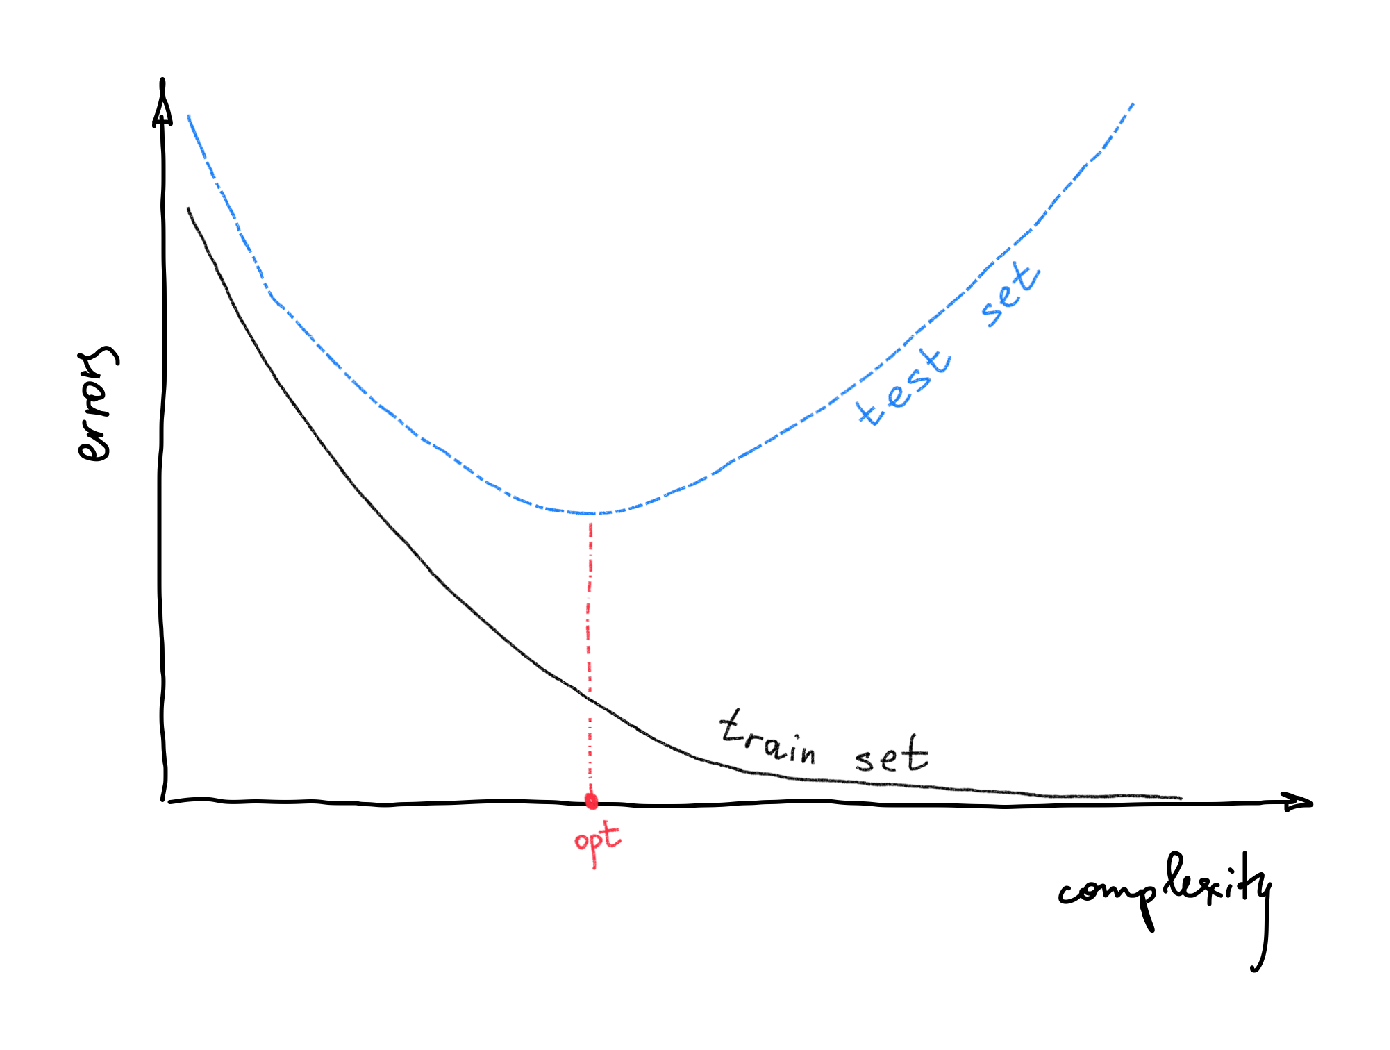
\includegraphics[width=1\columnwidth]{pics/choise_of_model.pdf}
    \caption{\emph{Выбор модели:} по оси абсцисс лежат модели (например, это могут быть степени аппроксимирующих многочленов), по оси ординат отмечается ошибка. Выбирается та модель у которой достигается наименьшая ошибка на тестовой выборке (на рисунке точка opt).}
    \label{fig:choise_of_model}
\end{marginfigure}
Общая рекомендация относить в тестовую выборку до 30\% всех данных. Методику с train-test'ом используют чтобы выбрать модель которой. Например, в задаче регрессии нужно понять многочленами какой степени стоит аппроксимировать данные. Отбирается та модель которая на тестовой выборке показывает минимальную ошибку. В цлеом это так или иначе упирается в кросс-валидацию.

\begin{itemize}
    \setlength\itemsep{0em}
    \item Обучащающая выборка - для обучения модели
    \item Тестовая выборка - для замера качества модели
    \item Валидационная выборка - для подбора гиппер-параметров
\end{itemize}

Альтернативой к валидации является подход с регуляризацией.

\section{Ящик с усами}

\begin{marginfigure}
    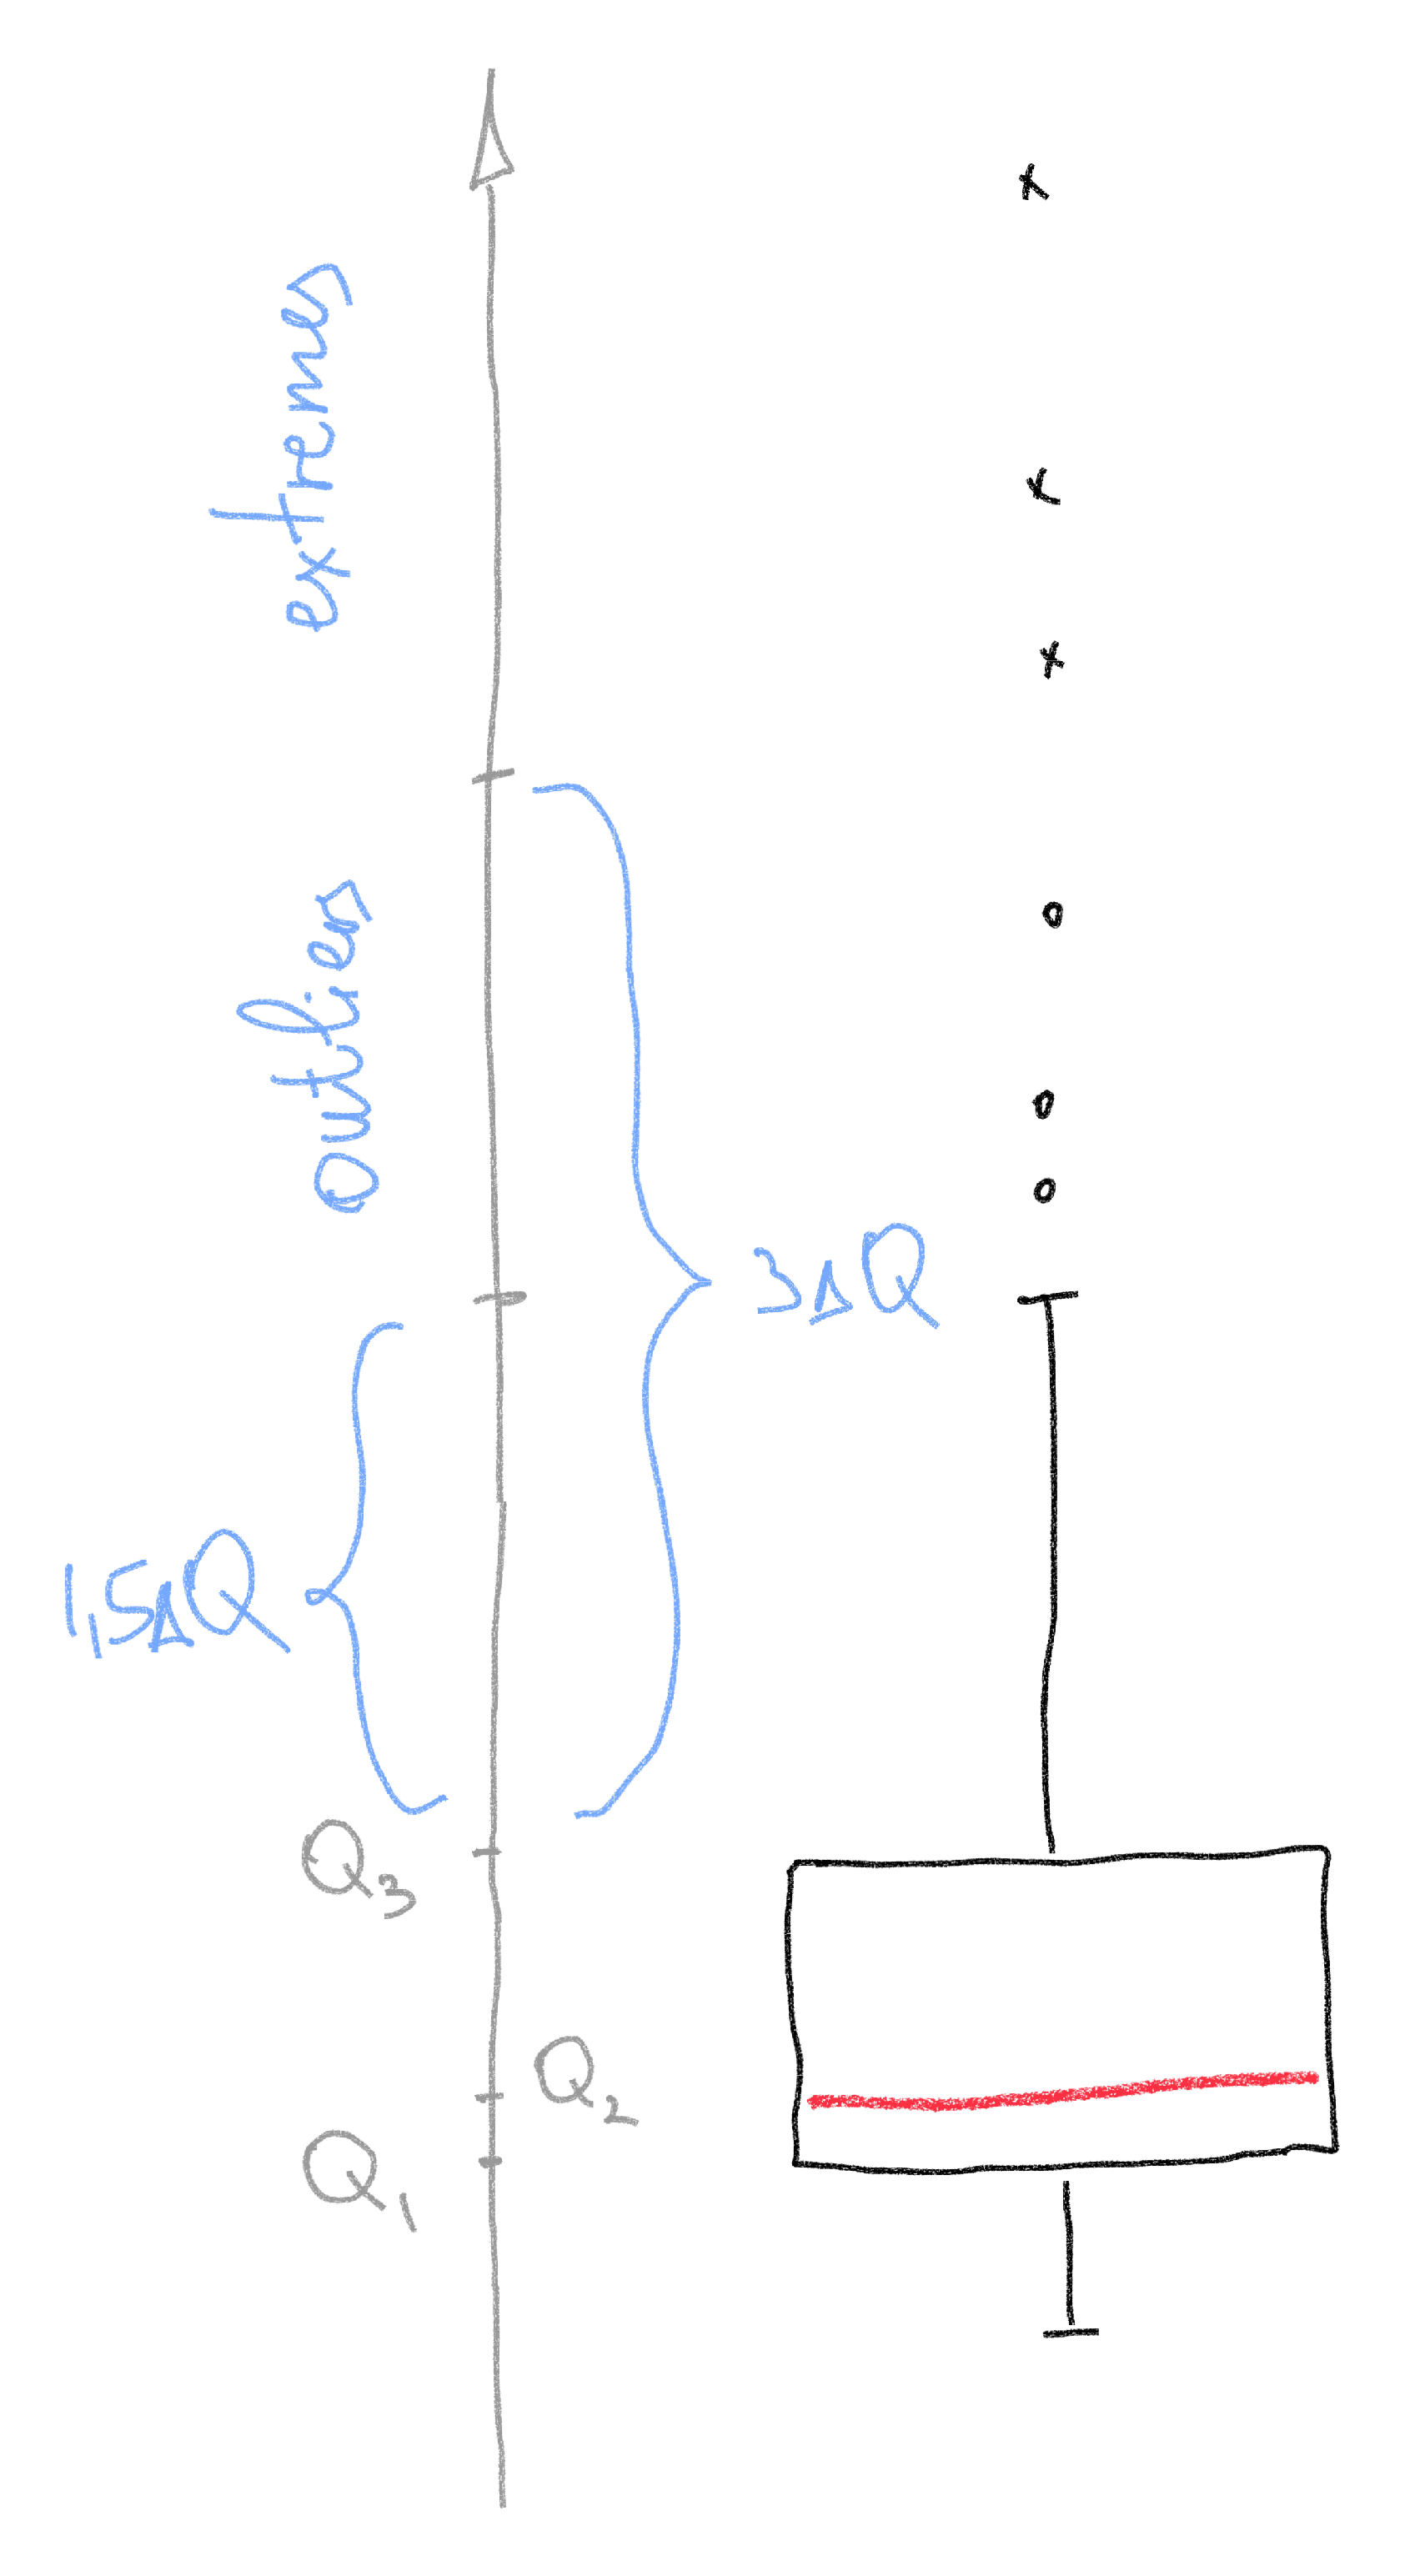
\includegraphics[width=2.7\columnwidth,angle=90]{pics/boxplot.pdf}
    %\caption{Движение $y$}
    \label{fig:boxplot}
\end{marginfigure}

Есть набор наблюдений $x_1, \dots, x_n$, По набору можно вычислить:
\begin{itemize}
    \item $\min$ - минимальное наблюдение
    \item $\max$ - максимальное наблюдение
    \item $M$ - медиана
    \item $Q_1$ - первый квартиль (25\%)
    \item $Q_3$ - третий квартиль (75\%)
\end{itemize}

\emph{Межквартильный размах} задается разностью $\Delta Q = Q_3 - Q_1$.

Длина правого усика, это минимум между расстоянием от квартиля $Q_3$ до
максимального элемента и полутора полуторным межквартильным расстоянием.
Аналогично расчитывается длина правого усика.
\[l = \min(\max(x_i) - Q_3, 1.5 \Delta Q)\]
\[r = \min(Q_1 - \max(x_i), 1.5 \Delta Q)\]
Данные за усиками это \emph{выбросы}, а если они вышли за три межвартильных
расстояния это \emph{чрезвычайные выбросы}.

В ящике с усами используется медиана вместо матожидания\marginpar{Усеченное
    среднее. Если из выборки удалить 2,5\% самых маленьких наблюдений и 2,5\%
    самых больших, то выбросы уже не так сильно будут влиять на вычисленное
матожидание.} в качестве описания потому, что она устойчива к
выбросам.

\chapter{Статистические гипотезы}

\section{Ошибки, значимость, p-value}

\begin{margintable}
    \caption{Ошибки I-го и II-го рода}
    \label{tab:mistakes}
    \begin{center}
        \begin{tabular}[c]{c|c c}
            {\it гипотеза} & верна & не верна \\
            \hline
            принята & + & {\it II род} \\
            отвергнута & {\it I род} & + \\
        \end{tabular}
    \end{center}
\end{margintable}

Если мы хотим опровергнуть какое-то утверждение, мы должны сформулировать
альтернативную гипотезу. Основная гипотеза всегда обозначается $H_0$,
альтернативная $H_1$. Основная гипотеза всегда должна быть простой, каким-то
конкретным утверждением, альтернативная может быть каким угодно. Такое
требование создается потому, что у нас нет мат.аппарата на сложные условия.

Влиять мы можем только на ошибку I-го рода. Ее обычно фиксируют на уровне 0,05,
0,01 или 0,005, но этот уровень можно менять на любой другой если этого требует
задача.

Ошибки второго рода контролировать сложнее. Для их уменьшения стараются
пользоваться состоятельными критериями.\marginpar{Критерий проверки гипотезы
называется состоятельным, если ошибка второго рода уменьшается с ростом числа
наблюдений.}

\begin{marginfigure}
    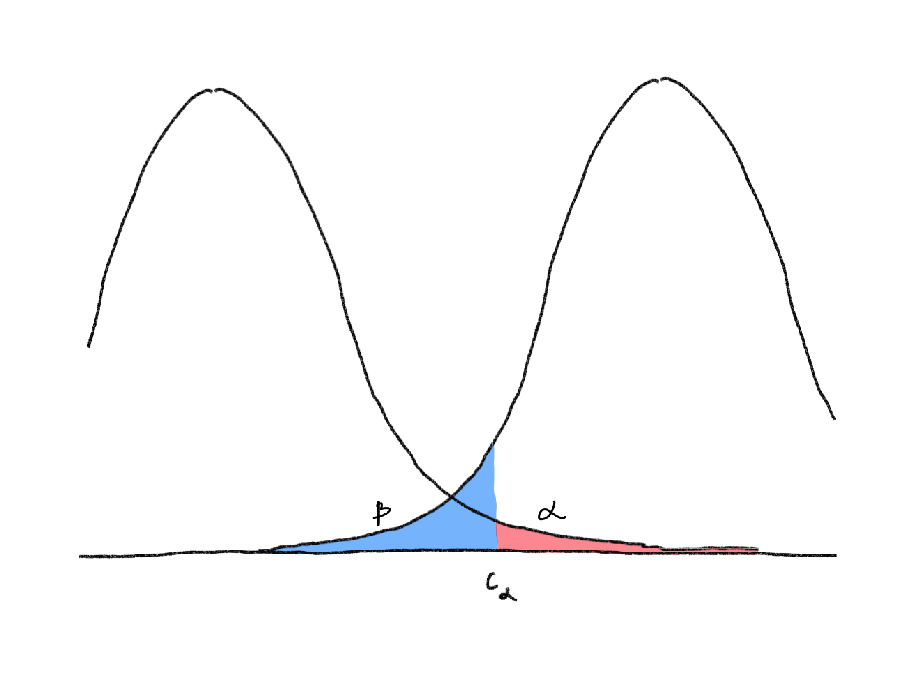
\includegraphics[width=1.1\columnwidth]{pics/critical_points_mistakes_value.pdf}
    \caption{Левое распределение соответствует гипотезе $H_0$, правое - гипотезе $H_1$.}
    \label{fig:crit_point}
\end{marginfigure}
Критическая точка критерия это такое значение вероятность превысить которое
равняется~$\alpha$ то есть вероятности ошибки первого рода. На рисунке
\ref{fig:crit_point} это площадь под графиком выше критической точки окрашенная
в красный. Синим обозначена вероятность ошибки II-го рода. Как видно это
вероятность получить выборку при которой не отвергается нулевая гипотеза, но
была верна альтернативная гипотеза.\marginpar{Проверять
    статистические гипотезы можно только в случае массовых явлений. События
    которые редки стат.гипотезами не проверяются. Число в 30 наблюдений
    считается достаточным только для нормальных распределений, для всех
    остальных надо больше данных.}

Критическая точка не обязана лежать на пересечении плотностей распределений
двух гипотез. Она определяется исходя только из плотности для нулевой гипотезы.

Альтернативой к механике проверки гипотез с критической точкой является
проверка гипотез через p-value. P-value вычисляется из предположения, что
нулевая гипотеза верна и определяет вероятность получить такое же значение
критерия или более экстремальное. Нам все равно нужно фиксировать уровень
значимости~$\alpha$ до эксперимента, но не нужно вычислять критическую точку.
Если p-value оказалось меньше~$\alpha$ то нулевая гипотеза должна быть
отвергнута, в противном случае нет оснований отвергать нулевую гипотезу.

\subsection{Ошибка подглядывания}
Ошибка подглядывания возникает когда мы заглядываем в результаты теста до
окончания самого теста (в промежуточное время). В этот момент человек может
увидеть промежуточный результат p-value~$< \alpha$. Во время подглядывания
может возникнуть соблазн дождаться когда p-value упадет ниже уровня
стат.значимости и остановить эксперимент. На самом деле график p-value в
процессе эксперимента может несколько раз опускаться ниже стат.значимости. Это
будет происходить случайно.\sidenote{\fullcite{karpov:ab_peeping}}

\marginpar{{\bf Процедура статистического тестирования:}
    \begin{enumerate}
        \item Определить метрику которую проверяем.
        \item Сформулировать нулевую и альтернативную гипотезы.
        \item Зафиксировать уровень стат.значимости~$\alpha$.
        \item Предрасчитать объем необходимой выборки для теста.
        \item Предрасчитать длительность теста.
        \item Запуск теста. В промежуточные результаты не заглядываем.
        \item По истечению времени, интерпретация результатов.
    \end{enumerate}

    Такая процедура обеспечит, что из всей массы запущенных экспериментов ошибки I рода будут наблюдаться с вероятностью~$\alpha$.
}

В случае если \emph{нулевая гипотеза верна}, вероятность получить p-value на
определенном уровне имеет равномерное распределение. Например, вероятность
получить p-value из первого дециля равна 10\%, вероятность получить p-value из
второго дециля это $P(\text{p-value} < 0.2) - P(\text{p-value} < 0.1) = 0.1$
тоже 10\%. Это означает, что отвергать нулевую гипотезу, то есть совершать ошибку I рода, мы будем с вероятностью~$\alpha$. 

Если же следить за p-value пока он не опустится ниже~$\alpha$ мы увеличим вероятность ошибки I рода и перестанем ее контролировать. И по сути будем выдавать желаемое за действительное.

\section{bootstrap}
Довольно мощный тест который позволяет вычислить параметры распределения или
какие-то дополнительные метрики по выборке.\marginpar{
    \it Bootstrap предполагает, что начальная выборка из которой мы производим
    сэмплирования является \emph{репререзентативной}.
}

Положим, что у нас какая-то \emph{репрезентативная} выборка~$S$ и мы хотим
оценить некоторый параметр~$\nu$. Например, это может быть первый квартиль или
разность матожиданий. 

Чтобы провести bootstrap проведем~$X(> 1000)$ раз процедуру:
\begin{enumerate}
    \item Просэмплируем из множества~$S$ подвыборку~$N$ элементов с возвращениями. На практике достаточно $50 < N < 100$.
    \item Посчитаем на полученной подвыборке параметр~$\nu$.
\end{enumerate}
В итоге мы получаем новую выборку из $X$ оценок параметра~$\nu$ и теперь можем оценить и как матожидание этого параметра, так и его доверительный интервал.

\section{Нормальность}
\marginpar{
    {\bf Преобразование Бокса-Кокса} это преобразование исходного набора
    данных. Применяют в основном с целью устранения выбросов. Например,
    при~$\lambda = 0$ это обычное логарифмическое преобразование.

    \[
        x_{i,\lambda} = 
        \begin{cases}
            \frac{x_i^\lambda - 1}{\lambda} & \text{если } \lambda \ne 0, \\
            \log(x_i) & \text{если } \lambda = 0.
        \end{cases}
    \]

    Параметр~$\lambda$ подбирается методом оптимизации правдоподобия.
}
\marginpar{
    {\it Почему такая формула?} Логарифмическое преобразование хорошо себя
    зарекомендовало, но оно не всегда справляется. Замечено, что $(\log x)' =
    \frac1x$. Преобразование Бокса-Кокса это обобщение до функций чьи
    производные равны $\frac{1}{x^\lambda}$.

}
Проверять данные на нормальность стоит не слишком тщательно. Данным достаточно только \emph{напоминать} нормальные, чтобы использовать большинство критериев в которых подразумевается, что данные нормальные. Если подходить к проверкам строго, то ничто и никогда невозможно будет проверить. 

Точно необходимо проверить:
\begin{enumerate}
    \item Выбросы. Отсутствие выбросов достаточно критичное условие. Если в данных есть выбросы, то их нельзя считать нормальными. С другой стороны если эти выбросы убрать, возможно уже можно будет работать.

    \item Асимметрия. Нормальные данные должны быть симметричными, поэтому если наблюдается асимметрия, то данные не нормальные. Возможно сможет помочь логарифмирование. 

    \item Отклонение от колоколообразности. Пограничным случаем колоколообразности можно считать равномерное распределение, а вот бимодальность гистограммы уже явный признак, что данные не нормальны. Еще чем больше наблюдений в данных, тем все-таки ближе должна быть гистограмма к нормальному распределению. За критерий можно взять выборку в $n=150$, чей график должен быть похож на колокол.
\end{enumerate}

Если в выборке менее 2000 объектов, то применяется метод Шапиро-Уилка, если же объектов больше, то используется критерий согласия Колмогорова-Смирнова.

\section{Доверительные интервалы}

Оценка показателей по выборке из генеральной совокупности всегда будет точечной оценкой. И если выбрать другую выборку, то оценка изменится. Чтобы учесть этот эффект вводят интервальную оценку показателя. 

\marginpar{$\alpha$ - уровень стат.значимости \\ $\beta$ - уровень доверия}
\emph{Доверительный интервал} для показателя~$\nu$ это такой интервал $(\nu_l, \nu_r)$ в который истинный показатель входит с вероятностью $\beta = 1 - \alpha$. 

\paragraph{Доверительный интервал для мат.ожидания} строится исходя из препосылки, что распределение измерений матожиданий по различным выборкам из генеральной совокупности должно уложиться в нормальное распределение. Отсюда мы можем вычислить радиус доверительного интервала такими формулами
\begin{equation}
    \label{eq:m_confidence_interval}
    \Delta = \frac{s}{\sqrt{n}} \; z_\alpha
    \qquad\text{или}\qquad
    \Delta = \frac{s}{\sqrt{n}} \; t_\alpha(n-1)\;.
\end{equation}
Критерий выбирается исходя из количества наблюдений или каких-то других особенностей прода. Также вместо выборочного ср.кв.отклонения можно использовать и истинную дисперсию если она известна, как правило это большая редкость.

% Эту же формулу~\ref{eq:m_confidence_interval} можно использовать для вычисления
достаточного объема выборки. Если мы знаем максимальное расстояние которое
может достигать доверительный интервал, то остается только обернуть формулу.
Радиус подбирают таким, чтобы конкурирующая гипотеза не входила в интервал.

\paragraph{Доверительный интервал для доли.}
\marginpar{
    Поскольку каждое изменение в выборке независимо, а объем выборки можно
    считать константой, можем сказать, что 
    \[ M[p\rbrack = M\lbrack k / n\rbrack  = M\lbrack k  / n\rbrack = np / n = p. \]
    Если учесть, что $ D\lbrack k \rbrack = npq $ и независимость выборки, получим
    \[ 
        D\lbrack p\rbrack =
        D\lbrack k / n\rbrack =
        D\lbrack k \rbrack / n^2 =
        npq / n^2 = pq / n.
    \]
}
Относительная частота события~$A$
вычисляется отношением $p = k / n$, где~$k$ --- число появлений события~$A$,
$n$ --- объем выборки. Тогда если учесть, что
\begin{equation}
    \label{eq:params_p_m_s}
    M[p] = p \qquad\text{и}\qquad D[p] = pq / n \,,
\end{equation}
можем воспользоваться формулой на вычисления вероятности интервала добавив еще уровень стат.значимости
\begin{equation}
    \label{eq:interval_prob_p}
    P(|X - k| < r) = 2\Phi(r / \sigma) = \alpha \,,
\end{equation}
откуда получим
\begin{equation}
    \label{eq:confidenc_interval_freq}
    r = z_\alpha \cdot \sqrt{\frac{p(1 - p)}{n}}
\end{equation}

Если нужно достать минимальный объем выборки, нужно знать заранее какой радиус~$r$ мы хотим обеспечить. Это можно определить исходя из потребности задачи (безнеса). Однако, есть еще один параметр который нужно знать заранее, это вероятность~$p$. Поскольку мы не знаем ее до эксперимента (получения выборки), можно положить $p = 0.5$. В этом случае выражение $p(1-p)$ примет наибольшее значение.


\section{Сравнение мат.ожиданий}
\marginpar{
    Для сравнения мат.ожиданий используются:
    \begin{itemize}
        \item t-критерий Стюдента
        \item Fligner-Killeen test
        \item Brown-Forsythe test
    \end{itemize}
}

\subsection{t-test, критерий Стьюдента}
Критерий Стюдента предполагает что метрика (н-р, матожидание) нормально распределена. Для двухвыборочного критерия важно равенство дисперсий. Так же тест не устойчив к выбросам в данных.

Одновыборочный тест\marginpar{
    Статистика для одновыборочного теста:\\
    $\overline x$ - выборочное матожидание \\
    $s^2$ - выборочная несмещенная оценка дисперсии \\
    $n$ - объем выборки
    \[H_0: M(x) = m\]
    \[t = \frac{\overline{x} - m}{s / \sqrt{n}}\]
    Степеней свободы $n-1$.
}
проводится когда у нас есть точное предположение о значении матожидания.

\paragraph{Двухвыборочный тест}
Предполагается, что есть две независимые выборки объема~$n_1$ и~$n_2$. Из
которых извлечены матожидания~$m_1$ и~$m_2$ и несмещенные дисперсии~$s_1^2$
и~$s_2^2$. 

\[H_0:m_1 = m_2\]

Если нулевая гипотеза верна, то разность $\Delta = m_1 - m_2$ имеет матожидание
$M(\Delta) = 0$\marginpar{
    Превращаем двувыборочный тест в одновыборочный!
}
и исходя из независимости выборок $D(\Delta) =
\frac{\sigma_1^2}{n_1} + \frac{\sigma_2^2}{n_2}$, так же получаем несмещенную
оценку разности выборочных средних $D(\Delta) = \frac{s_1^2}{n_1} +
\frac{s_2^2}{n_2}$. Теперь можем определить статистику

\begin{equation}
    \label{eq:t-test}
    t = \frac{m_1 - m_2}{\sqrt{\frac{s_1^2}{n_1} + \frac{s_2^2}{n_2}}}
\end{equation}

Степени свободы вычисляются по формуле
\begin{equation}
    \label{eq:t-test-degree}
    df = \frac{
        \left( \frac{s_1^2}{n_1} + \frac{s_2^2}{n_2}\right)^2
    }{
        (\frac{s_1^2}{n_1})^2/(n_1 - 1) + (\frac{s_2^2}{n_2})^2/(n_2-1)
    }
\end{equation}

\paragraph{Объем выборки.}
\marginpar{
    $1 - \beta$ --- мощность (power) \\
    $\delta = m_1 - m_0$ --- MDE
}

Чтобы рассчитать объем необходимой выборки для проведения теста нужно зафиксировать уровень ошибок второго рода~$\beta$. Критическая точка определяет границу между принятием нулевой гипотезы или альтернативной. Если посчитать границу исходя из каждой гипотезы получим такое уравнение

\marginpar{
    \[
        z = \frac{x - m}{s}  \quad\longrightarrow\quad
        x = m + z \cdot s
    \]
}
\begin{equation}
    \label{eq:sample_size_border}
    \cancel{m_0} + z_{1-\alpha / 2} \,s_0 \sqrt{\frac{1}{n_0} + \frac{1}{n_1}}
    = 
    \cancel{m_0} + \delta - z_{1-\beta} \,\sqrt{\frac{s_0}{n_0} + \frac{s_1}{n_1}}.
\end{equation}

Уравнение~\ref{eq:sample_size_border} основа для расчета минимального объема выборки. Если предположить $n_0 = n_1 = n$, что обеспечит одинаковый объем в тестовом и контрольном сплитах, и $\sigma_0 = \sigma_1 = \sigma$ поучим формулу
\marginpar{
    Chapter 2 in
    \fullcite{van2011statistical}
}
\begin{equation}
    \label{eq:sample_size_for_mean}
    n = \frac{s^2 (z_{1 - \alpha / 2} + z_{1 - \beta})^2}{\delta^2}
\end{equation}

% \marginpar{
    Величина~$\delta$ определяет минимальный обнаруживаемый эффект MDE (minimal
    detectable effect). В формуле~\eqref{eq:sample_size_for_mean} он
    присутствует в виде делителя. Это значит, что за обнаружение минимального
    профита нам придется заплатить увеличением выборки. 
% }

\section{Сравнение медиан}
\marginpar{
Для сравнения медиан используются:
\begin{itemize}
    \item Mood's median test. Только для гигантских данных. На малых данных будет большая ошибка 2 рода.
    \item критерий Мана-Уитни. Есть критика критерия, но крайние случаи довольно редкие и ими пренебрегают и все равно используют критерий.
\end{itemize}
}

\subsection{Критерий Манна-Уитни. U-test.}

\begin{marginfigure}
    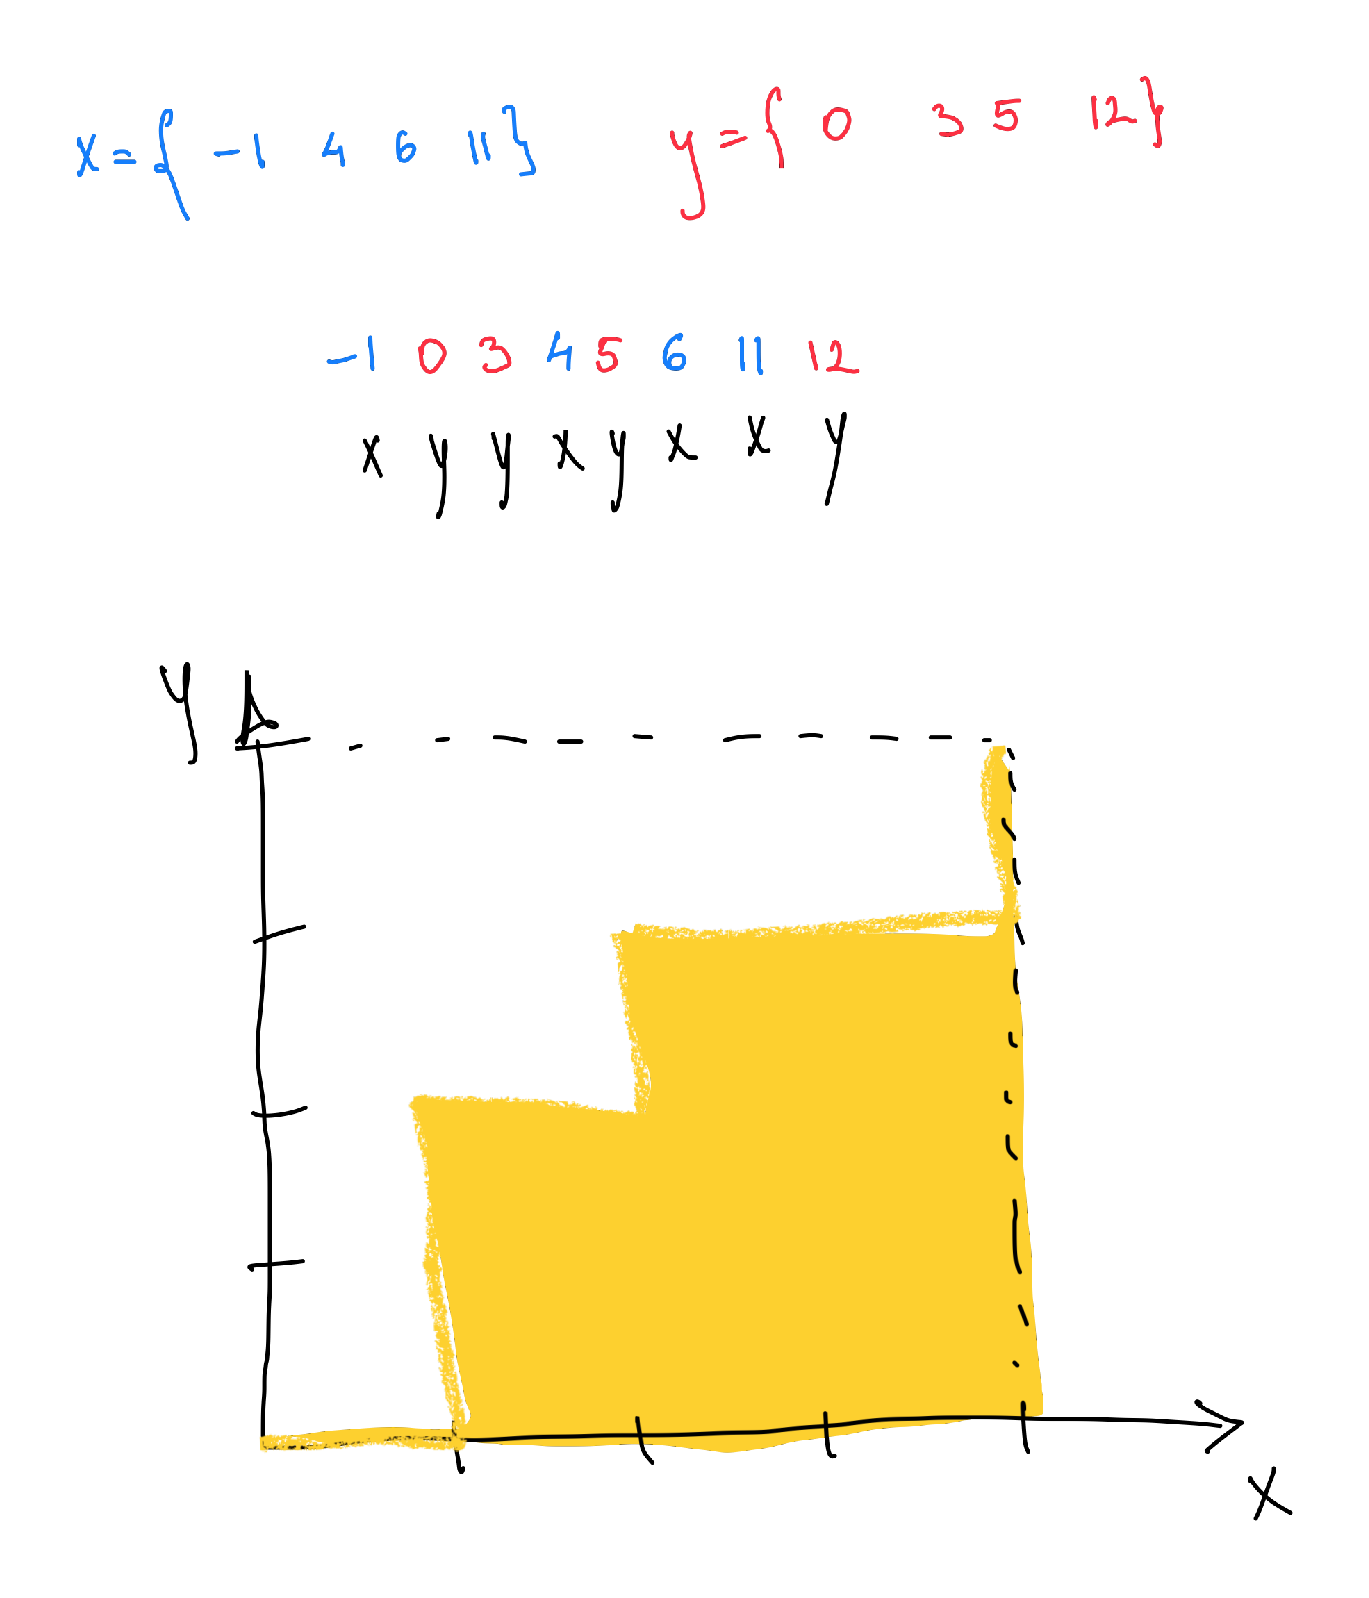
\includegraphics[width=1.1\columnwidth]{pics/mann-whitney_roc.pdf}
    \label{fig:mann-whitney_roc}
\end{marginfigure}
Чтобы применить критерий Манна-Уитни данные должны обладать порядком (числа
подходят). Это непараметрический тест поэтому область его применения может быть
шире, чем просто над числовыми показателями.

Положим есть две выборки $x_{i=\overline{1, n_1}}$ и~$y_{j=\overline{1, n_2}}$.
Тогда мы можем составить слово из букв~$X$ и~$Y$ последовательно вынимания из
объединения $x \cup y$ минимальный элемент. Буква определяется принадлежностью
множеству. Такую последовательность уже можно конвертировать в ROC кривую. Если
обе выборки принадлежат одному распределению, то буквы в слове перемешаются
равномерно, а значит кривая будет диагональю, площадь под которой равна
$S=\frac{n_1\,n_2}{2}$. Так мы свели задачу к проверки гипотезы о мат.ожидании.

\begin{itemize}
    \item[$H_0$:] Обе выборки из одной генеральной совокупности
    \item[$H_1$:] Выборки из разных генеральных совокупностей
\end{itemize}


Обозначим через $T_\ast$ сумму рангов элементов из разных выборок в объединении. Теперь мы можем посчитать
\begin{equation}
    \label{eq:Mann-Whitney:U}
    \left.
    \begin{array}{ll}
        U_x &= n_x \, n_y + \frac{n_x (n_x + 1)}{2} - T_x \\
        U_y &= n_x \, n_y + \frac{n_y (n_y + 1)}{2} - T_y
    \end{array}
    \;\right]
    \quad \Rightarrow \quad
    U = \min(U_x,\; U_y)
\end{equation}

\marginpar{MDE можно вычислять как для одновыборочного теста на мат.ожидание.}
\begin{equation}
    \label{eq:Mann-Whitney:z-value}
    \left.
    \begin{array}{ll}
        m_U &= n_x\,n_y / 2 \\ %\frac{n_x\,n_y}{2} \\
        s_U &= \sqrt{
            \frac{n_x\,n_y\,(n_x + n_y + 1)}{12}
        }
    \end{array}
    \;\right]
    \quad \Rightarrow \quad
    z = \frac{U - m_U}{s_U}
\end{equation}
\marginpar{\fullcite{watkins2019introduction}}




\section{Проверка зависимости}
При проверке зависимости между двумя случайными величинами используют коэффициенты корреляции:
\begin{itemize}
    \setlength\itemsep{0em}
    \item Пирсона, если данные нормальные.
    \item Спирмена, в остальных случаях.
    \item Кендела, очень редко.
\end{itemize}

При вычислении корреляций надо понимать, что они ищут только линейные зависимости, коэффициенты могут быть очень чувствительными к выбросам и иногда могут показывать ложную корреляцию, например, для монотонных временных рядов.

\chapter{Кластеризация}

\section{Кластерный анализ}
\begin{marginfigure}
    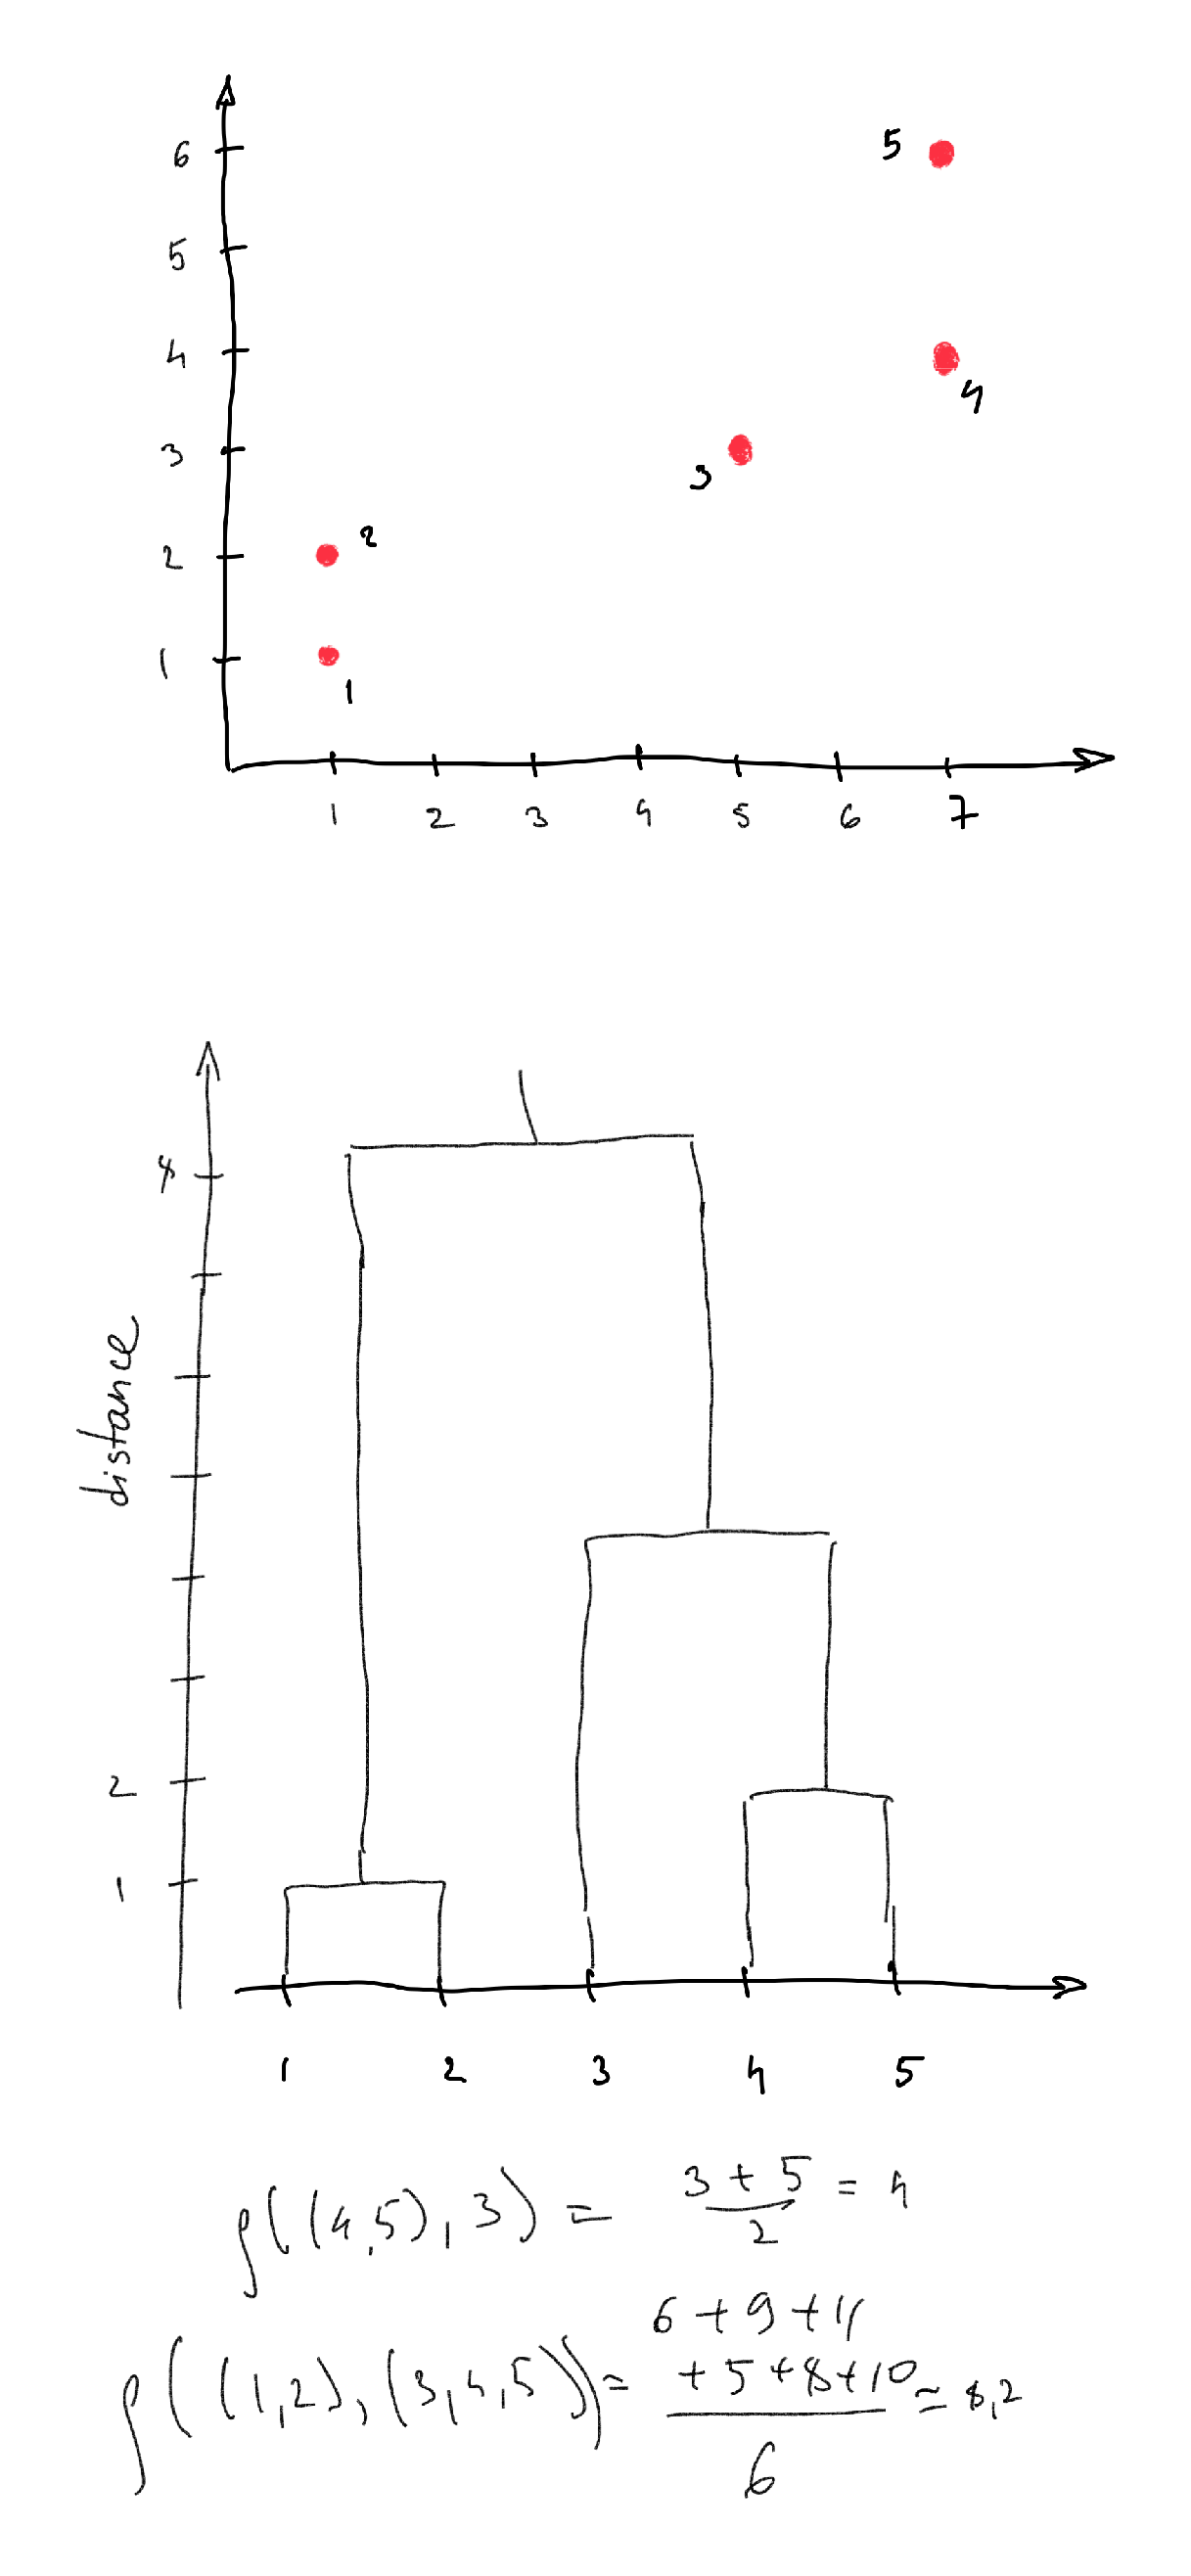
\includegraphics[width=1.1\columnwidth]{pics/dendrogram.pdf}
    %\caption{Движение $y$}
    \label{fig:boxplot}
\end{marginfigure}
Расстояния между кластерами могут быть заданы по разному и стоит обращать
внимание на решаемую задачу. Чтобы задать расстояние между кластерами надо
определить расстояние между точками и на ее основе определить метод построения
кластерного расстояния. Чаще всего используют такие методы:

\begin{itemize}
    \item среднее невзвешенное расстояние (average linkage clustering) -
        среднее расстояние между парами из различных кластеров

    \item центроид метод (устаревший) - расстояние между кластерами
        определяется как расстояние между центрами масс.

    \item метод дальнего соседа (complete linked clustering) - по расстоянию
        между максимально удаленными точками кластеров

    \item метод ближайшего соседа (single linkage clustering) - по расстоянию
        между самыми близкими точками

    \item метод Варда (Ward's method)
\end{itemize}

Дендрограмма выращивается снизу вверх. Сперва каждая точка представляет свой
собственный кластер. Если при достижении уровня $h$ расстояние между точками
равно $h$ то точки объединяются в один кластер (на рисунке это спайка). Процесс
повторяется до тех пор пока не останется один единственный кластер.

Для определения количества кластеров используют метод \emph{плеча}. Для этого
строится график где по оси абсцисс отмечаются шаги объединения (первое
объединение, второе и так далее), по оси ординат откладывается высота на
котором произошло объединение кластеров. На графике ищется точка перелома,
когда расстояние резко увеличивается. Это количество кластеров в данных по
методу локтя.
\marginpar{Результаты кластерного анализа нужно интерпретировать: анализ всегда
должен давать что-то новое о данных, что общего у объектов в кластере и чем
различаются кластеры.}
\marginpar{
    Кривую локтя можно построить и для метода k-средних. В этом случае по оси
    абсцисс будет лежать выбранный $k$ по оси ординат качество получившейся
    кластеризации.

    См. \fullcite{yandex:book}, глава 7.
}

Недостатки иерархической кластеризации:
\begin{itemize}
    \item Плохо справляется с данными которые вытянуты в длинные ленты в
        простраснтве

    \item Для вычисления требуется хранить попарные расстояния между объектами.
\end{itemize}

\section{DBSCAN}
Density-based spatial clustering of applications with noise. Сильный
топологический алгоритм. Основан на поиске связных компонент в покрытии данных
$\epsilon$-шарами. Количество кластеров определяет автоматически.

Все объекты в наблюдениях делятся на три категории:
\begin{itemize}
    \item core point (внутренние / основные) - если в окрестности есть более
        $N_0$ соседей

    \item border point (граничные) - если в окрестности меньше $N_0$ внутренних

    \item noise point (шумовые) - если в окрестности нет внутренних точек.
        Автоматически содержат меньше $N_0$ объектов.
\end{itemize}

Алгоритм DBSCAN:
\begin{marginfigure}
    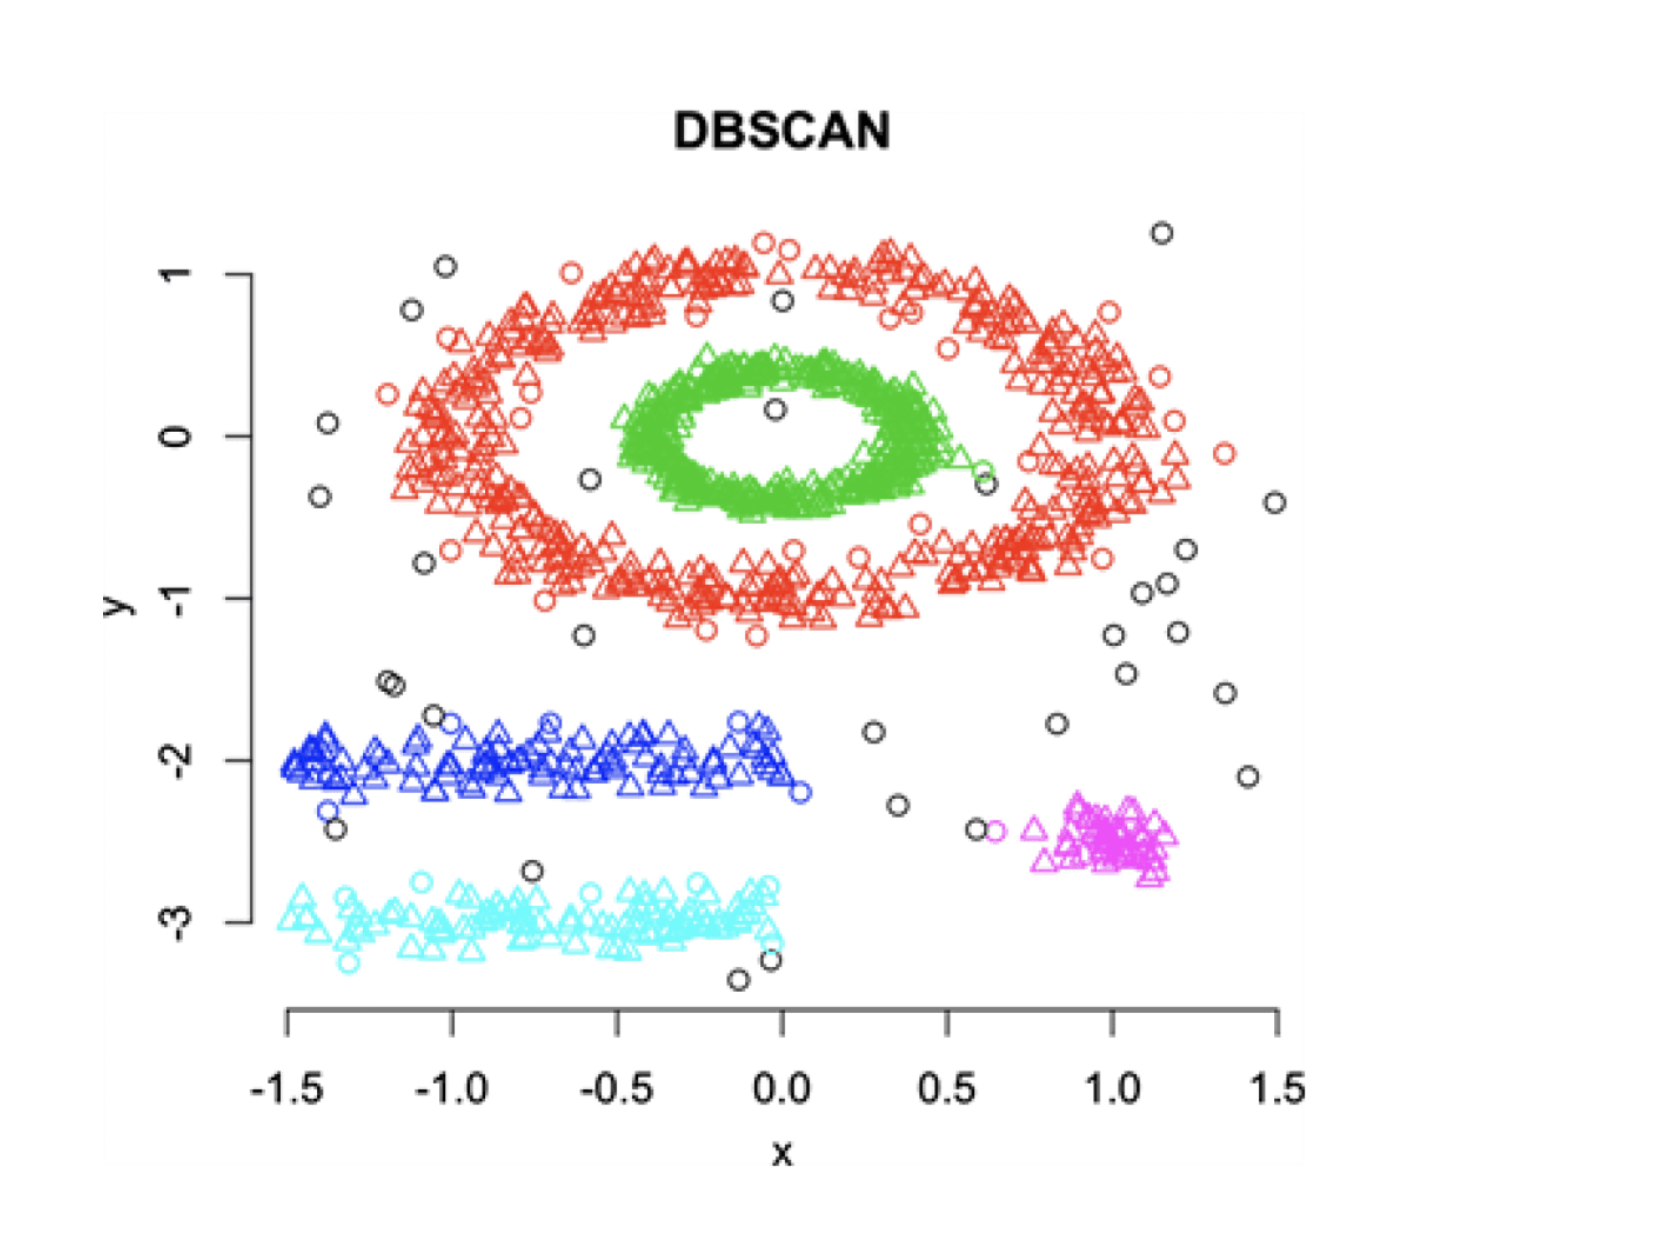
\includegraphics[width=1.3\columnwidth]{pics/dbscan.jpeg}
    %\caption{Движение $y$}
    \label{fig:boxplot}
\end{marginfigure}
\begin{enumerate}
    \item Шумовые точки удаляются из рассмотрения и не приписываются ни какому
        кластеру.

    \item Основные точки у которых есть общая окрестность соединяются ребром.
        Строится граф.

    \item В полученном графе вычисляются компоненты связности.

    \item Каждая граничная точка относится к тому кластеру, в который попала
        ближайшая к ней внутренняя точка.
\end{enumerate}

\chapter{Классификация и регрессия}

\section{Линейная регрессия}
\begin{marginfigure}
    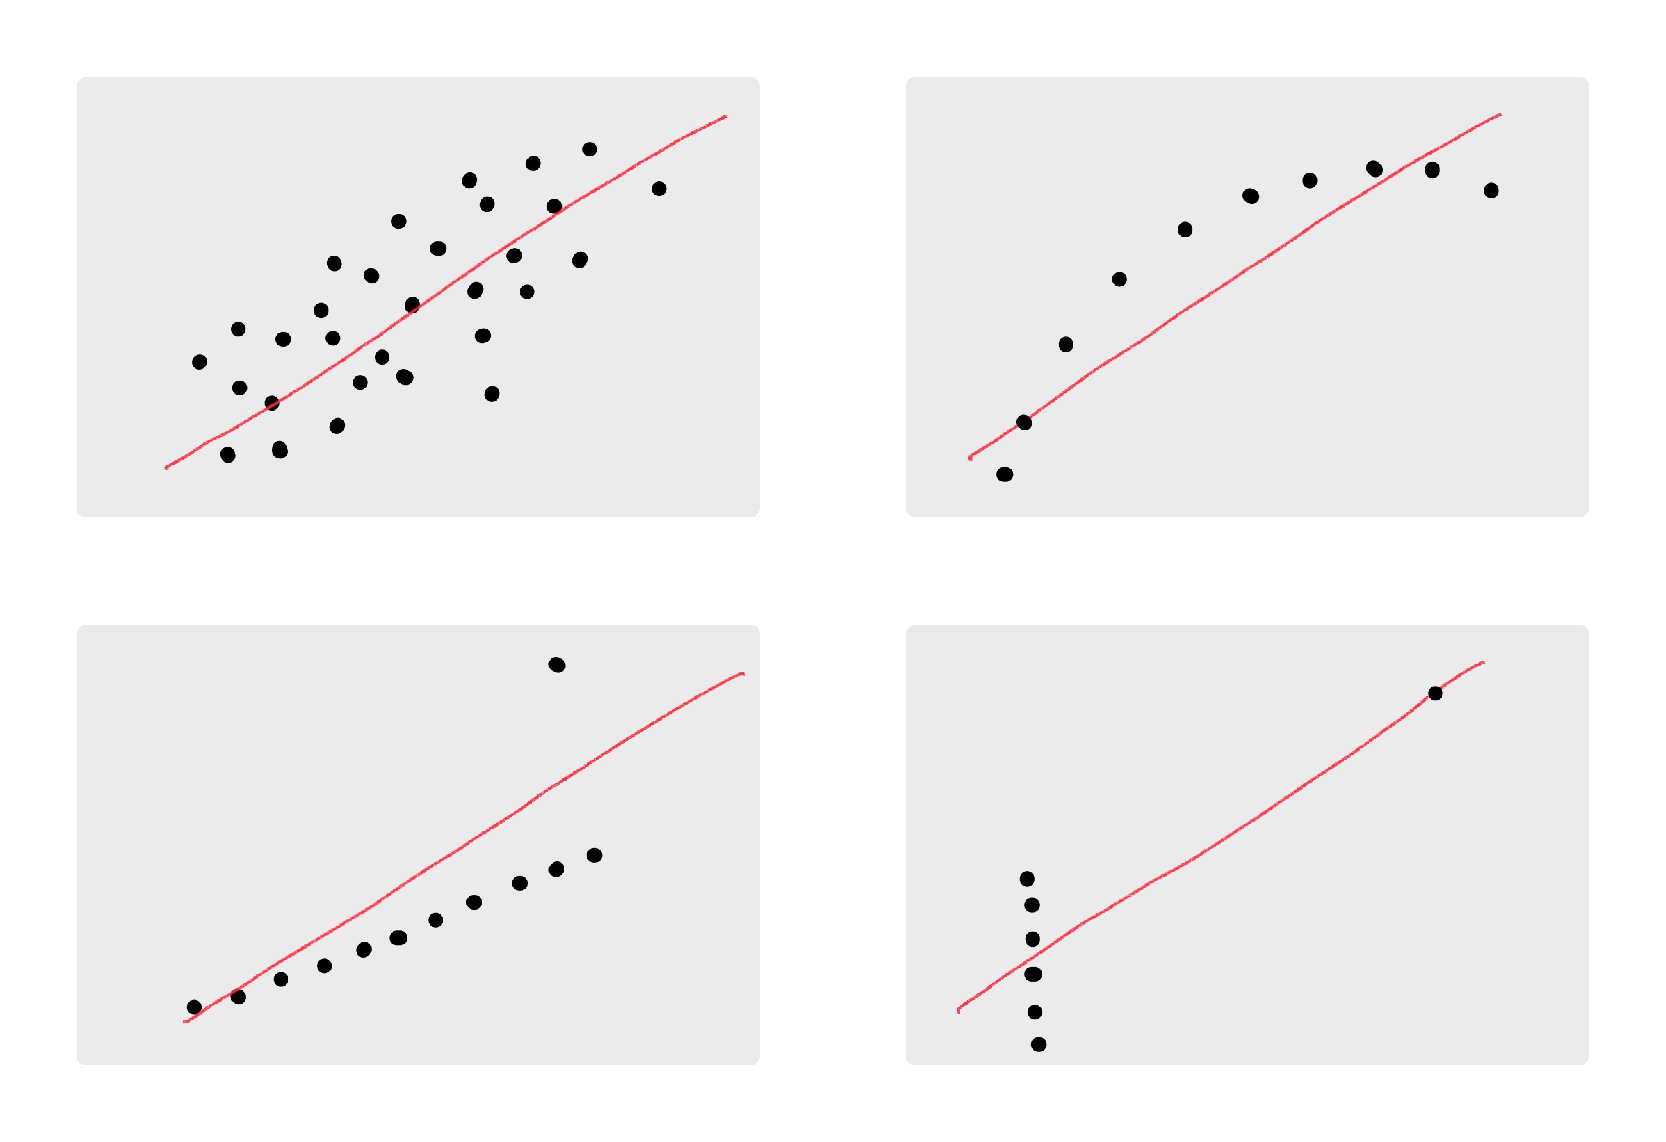
\includegraphics[width=1\columnwidth]{pics/anscombe_quartet.pdf}
    \caption{Квартет Анскомба. Иллюстрация как линейная регрессия может лажать. Для данных подобрали не ту модель или в данных есть сильные выбросы - все приводит к некорректному построению регрессии.}
    \label{fig:anscombe}
\end{marginfigure}

Для Определения на сколько модель хороша используют коэффициент детерминации. Чтобы его вычислить нужна обученная модель.
\begin{equation}
    \label{eq:coeff_of_determination}
    R^2 = 1 - \frac{D[y|x]}{D[y]}
\end{equation}
В сущностной части это на сколько дисперсия предсказания отличается от дисперсии наблюдений.

\marginpar{
    \emph{Наивная мультивариантная линейная регрессия:}
    \[ y = X\beta + \epsilon\]
    \[\epsilon \sim N(0,\, \sigma^2 I)\]
    $\epsilon$ - коэффициент \emph{невязки}, определяет шум системы.

    Коэффициенты находятся формулой
    \[ \hat \beta = (X^TX)^{-1}X^Ty \]

    Вариация вычисленных коэффициентов
    \[ Var(\hat \beta) = \sigma^2 (X^TX)^{-1}\]
    Это легко вывести если воспользоваться формулой дисперсии произведения 
    \[Var(AX) = A \cdot Var(X) \cdot A^T.\]
}

Во время построения модели регрессии самая большая проблема - наличие коллинеарных векторов (зависимых переменных в фичах). Чтобы очистить список фичей, можно проверить гипотезу что вычисленная фича нулевая (для каждой фичи индивидуально). 

\begin{equation*}
    \label{eq:zero_coeff_hyp}
    \left\{
    \begin{array}{lr}
        H_0: & \; \hat \beta_i = 0 \\
        H_1: & \; \hat \beta_i \ne 0
    \end{array}
    \right.
\end{equation*}

Если предположить что коэффициент имеет нормальное распределение, то мы можем
воспользоваться t-тестом Стьюдента и посчитать p-value. Если гипотеза не будет
отвергнута, это будет означать, что мы фичу стоит выкинуть потому что ее
коэффициент равен нулю. Соответственно там где гипотеза не подтвердилась фичи
являются ценными.

Выкидывать фичи стоит по одному. Начиная с самой слабой по p-value, каждый раз
с новым набором фичей анализ лучше проводить заново.\sidenote{\fullcite{Watts:ItS}}

\subsection{Для временных рядов}
Линейная регрессия может быть очень полезной во временных рядах, когда мы наблюдаем в них несколько сезонностей или когда данных относительно мало, нет нескольких полных сезонов в данных.

Чтобы учесть сезонность во временных рядах создают фичи:
\begin{itemize}
    \setlength\itemsep{0em}
    \item 1 - свободный коэффициент, bias
    \item $\delta_s(t)$ - учет сезонности, бинарный признак, что дата/время $t$ попало во временной интервал~$s$  (час, день, неделя, месяц и пр).
\end{itemize}
При этом очевидно, что если сложить все фичи $\delta_s(t)$ сезонности мы получим свободную переменную, то есть на лицо линейная зависимость. 

\section{Деревяшки (решающие деревья)}

\marginpar{
    {\bf Обозначения:}
    \begin{description}
        \item $N$ --- объем выборки
        \item $D$ --- размерность признаков
        \item $y = \{ y_i \}_{i=1}^N \subset \mathbb{R}^N$ --- вектор таргетов
        \item $X = \{x_i\}_{i=1}^N \in \mathbb{R}^{N \times D}$ --- матрица признаков
    \end{description}

    %\[x_{\text{строка}}^{\text{столбец}}\]
}

Решающее дерево имеет в узлах предикаты, а в листьях метки классов или другие значения в зависимости от задачи.

Чаще всего строят бинарные решающие деревья и используют такие предикаты:
\begin{equation}
    \label{eq:tree_predicat}
    B(x, j, t) = [x^j \le t] = B_{j,t}(x)
\end{equation}

\marginpar{
    \emph{Impurity criterion (критерий информативности)}~$H(R)$ оценивает
    качество распределения целевой переменной в множестве~$R$. 

    Поскольку это про оценку распределения часто используют энтропию или индекс
    Джини, но также может использоваться и квадрат/модуль ошибок и прочее.
}

Если в вершине выбрано какое-то разбиение и множество $R$ было разбито на два $R_l$ и $R_r$ то можно почитать на сколько мы сделали лучше этим разбиением.\sidenote{\fullcite{sokolov:desigion_tree}}
\begin{equation}
    \label{eq:tree_split_quality}
    Q(R, B_{j,t}) = H(R) - \frac{| R_l |}{| R | } H(R_l) - \frac{| R_r |}{| R |}H(R_r)
\end{equation}


Чтобы выбрать лучший вариант разбиения условия разбиения по признаку~$j$ можно
упорядочить все наблюдения в узле по этому признаку постепенно перебрать все
варианты разбиений и выбрать тот в котором функция качества~$Q$ достигает
максимума. Эту процедуру повторяем для всех $j = \overline{1, D}$ и выбираем лучшее разбиение.

\begin{equation}
    \label{eq:opt_node_value}
    (j_{opt}, t_{opt}) = \argmax_{j, t} Q(R, B_{j,t})
\end{equation}

\marginpar{Если на тестовой выборке результат заметно хуже, а мы очень хотим обучить дерево, можно попробовать упростить модель, сильнее ограничить глубину дерева.}

\marginpar{
    Для решения \emph{задачи регрессии} достаточно подобрать критерий
    информативности. Например, это может быть квадрат отклонения от среднего

    \[
        H(R) = \frac{1}{|R|} \sum_{(x_i,\,y_i) \in R}
        \left(
            y_i - \frac{1}{|R|} \sum_{(x_i,\,y_i) \in R} y_i
        \right)^2
    \]
}

Для процедуры критерий останова можно вводить разными способами. Самые
популярные такие:
\begin{itemize}
    \setlength\itemsep{0em}
    \item максимальная глубина дерева,
    \item максимальное количество листьев,
    \item минимальное число объектов в листе,
    \item все объекты в листе лежат в одном классе,
    \item качество улучшилось не более чем на $x$ процентов.
\end{itemize}

Деревья дают кусочно-линейные решения, однако у них есть преимущества в том,
что они могут вытащить нелинейные зависимости; а также и недостатки, за
пределами наблюдений регрессия будет предсказываться константой. Другими
словами регрессия на деревьях не умеет экстраполировать, зато может быть
полезна в интерполяции.

\medskip
\printbibliography

\end{document}
